\subsection{Caso d'uso UC6: Ricerca e selezione questionario esistente}
\label{UC6}
\begin{figure}[h]
\centering
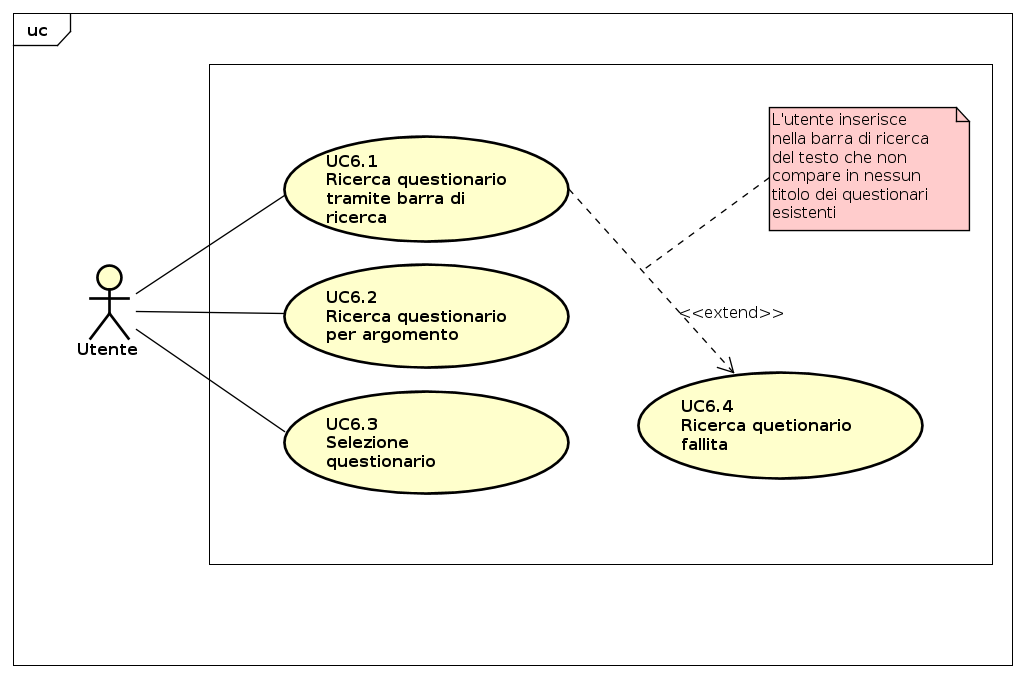
\includegraphics[scale=0.5,keepaspectratio]{UML/UC6.png}
\caption{UC6: Ricerca e selezione questionario esistente}
\end{figure}
\FloatBarrier
\begin{itemize}
\item\textbf{Attori Principali}: Utente non autenticato, Utente autenticato, Utente autenticato pro;
\item\textbf{Descrizione}: nella schermata principale qualsiasi utente che voglia svolgere un questionario potrà ricercarlo attraverso:
\begin{itemize}
\item la barra di ricerca tramite il titolo del questionario;
\item una suddivisione per argomento dei questionari esistenti.
\end{itemize}
Per poterlo compilare dovrà poi selezionare il questionario che ha scelto oppure se in quel momento non ha il tempo di farlo potrà inserirlo nella lista "Fai più tardi".	
\item\textbf{Precondizione}: l'utente si trova nella pagina principale dell'applicazione;
\item\textbf{Postcondizione}: l'utente ha selezionato il questionario che vuole svolgere;
\item\textbf{Scenario principale}:
\begin{itemize}
\item L'utente cerca un questionario tramite barra di ricerca (UC6.1);
\item L'utente cerca un questionario per argomento (UC6.2);
\item L'utente seleziona il questionario scelto (UC6.3);
\item L'utente aggiunge il questionario alla lista "Fai più tardi"(UC6.4);
\end{itemize}
\item\textbf{Scenario alternativo}: L'utente inserisce nella barra di ricerca del testo che non compare in nessun titolo dei questionari esistenti;
\item\textbf{Estensioni}: Ricerca questionario fallita (UC6.5).
\end{itemize}

\subsubsection{Caso d'uso UC6.1: Ricerca questionario tramite barra di ricerca}
\begin{itemize}
\item\textbf{Attori Principali}: Utente non autenticato, Utente autenticato, Utente autenticato pro;
\item\textbf{Descrizione}: all'interno della pagina principale dell'applicazione è presente una barra di ricerca dove è possibile cercare, attraverso il titolo, un determinato questionario;
\item\textbf{Precondizione}: l'utente si trova nella pagina principale dell'applicazione;
\item\textbf{Postcondizione}: l'utente visualizza i questionari che hanno nel titolo il testo che ha scritto nella barra di ricerca;
\item\textbf{Scenario principale}: l'utente utilizza la barra di ricerca per cercare un questionario del quale conosce il titolo o parte di questo;
\end{itemize}

\subsubsection{Caso d'uso UC6.2: Ricerca questionario per argomento}
\begin{itemize}
\item\textbf{Attori Principali}: Utente non autenticato, Utente autenticato, Utente autenticato pro;
\item\textbf{Descrizione}: all'interno della pagina principale dell'applicazione è presente una sezione contenete tutti i questionari esistenti suddivisi per argomento trattato;
\item\textbf{Precondizione}: l'utente si trova nella pagina principale dell'applicazione;
\item\textbf{Postcondizione}: l'utente visualizza un insieme di questionari suddivisi per argomento;
\item\textbf{Scenario principale}: l'utente che non conosce i questionari esistenti, si reca nella sezione in cui sono suddivisi per argomento in modo da rendere più facile la scelta di uno di questi. 
\end{itemize}

\subsubsection{Caso d'uso UC6.3: Selezione questionario}
\begin{itemize}
\item\textbf{Attori Principali}: Utente non autenticato, Utente autenticato, Utente autenticato pro;
\item\textbf{Descrizione}: l'utente dopo aver scelto un questionario, per iniziare a compilarlo, deve selezionarlo;
\item\textbf{Precondizione}: l'utente ha scelto il questionario che vuole svolgere;
\item\textbf{Postcondizione}: l'utente ha selezionato il questionario scelto;
\item\textbf{Scenario principale}: l'utente conferma la selezione del questionario (UC6.3.1);
\item\textbf{Scenario alternativo}: l'utente cambia idea e annulla l'operazione tornando alla schermata precedente.
\end{itemize}

\subsubsection{Caso d'uso UC6.3.1: Conferma selezione questionario}
\begin{itemize}
\item\textbf{Attori Principali}: Utente non autenticato, Utente autenticato, Utente autenticato pro;
\item\textbf{Descrizione}: l'utente conferma la selezione del questionario, potendo così procedere con la compilazione;
\item\textbf{Precondizione}: ;
\item\textbf{Postcondizione}: l'utente ha confermato la selezione del questionario;
\item\textbf{Scenario principale}: l'utente conferma di voler svolgere il questionario selezionato.
\end{itemize}

\subsubsection{Caso d'uso UC6.4: Aggiungi a "Fai più tardi"}
\begin{itemize}
\item\textbf{Attori Principali}: Utente autenticato, Utente autenticato pro;
\item\textbf{Descrizione}: l'utente che sta cercando dei questionari da svolgere, può decidere di aggiungere alla personale lista "Fai più tardi" i questionari che sta visualizzando, potendoli recuperare così in seguito;
\item\textbf{Precondizione}: l'utente ha cercato dei questionari;
\item\textbf{Postcondizione}: l'utente ha aggiunto il questionario alla lista "Fai più tardi";
\item\textbf{Scenario principale}: l'utente che in quell'istante non può svolgere certi questionari che sta visualizzando, li può aggiungere alla personale lista "Fai più tardi".
\end{itemize}

\subsubsection{Caso d'uso UC6.5: Ricerca questionario fallita}
\begin{itemize}
\item\textbf{Attori Principali}: Utente non autenticato, Utente autenticato, Utente autenticato pro;
\item\textbf{Descrizione}: L'utente ha inserito nella barra di ricerca del testo che non compare in nessun titolo dei questionari esistenti;
\item\textbf{Precondizione}: l'utente ha utilizzato la barra di ricerca per cercare un questionario che non esiste;
\item\textbf{Postcondizione}: il sistema avvisa l'utente dell'errore verificatosi tramite un opportuno messaggio;
\item\textbf{Scenario principale}: l'utente visualizza un messaggio che lo avvisa del mancato ritrovamento di questionari;
\end{itemize}